\documentclass[tikz,margin=1mm]{standalone}
\usepackage{xcolor,amsmath}

 \usetikzlibrary{arrows.meta,chains, decorations.pathreplacing,bending,positioning}



\begin{document}
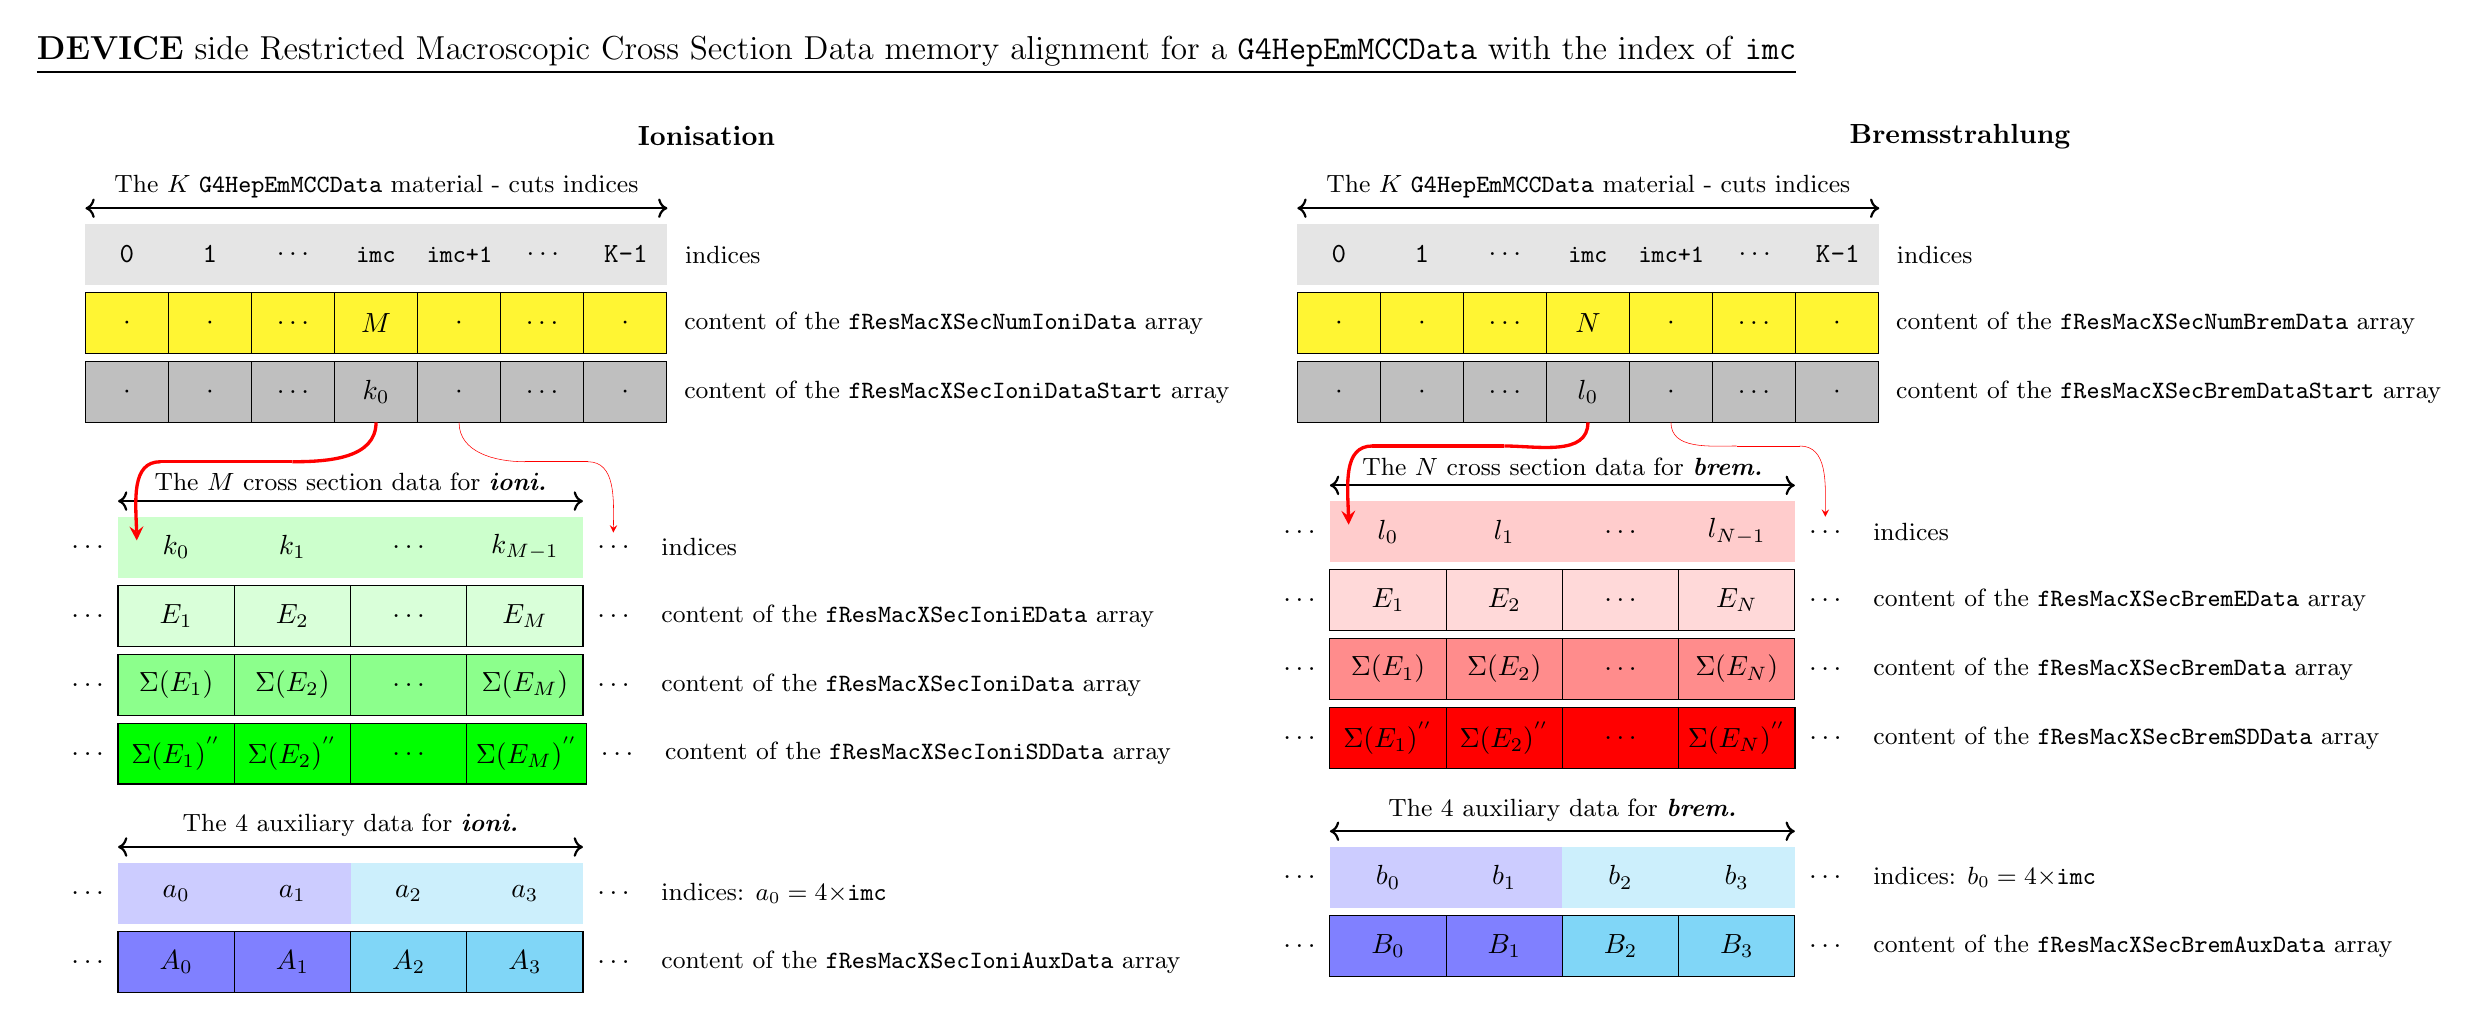
\begin{tikzpicture}[
   start chain       = going right,
   node distance = 0pt,
    %
   noStyle/.style  = {draw=none, minimum width=2.2em, minimum height=2.2em, outer sep=0pt, font=\ttfamily, on chain},
   %
   eiStyle1/.style  = {draw=none, minimum width=3.0em, minimum height=2.2em, outer sep=0pt, font=\ttfamily, on chain, fill=yellow!30},
   eStyle1/.style   = {draw, minimum width=3.0em, minimum height=2.2em, outer sep=0pt, on chain, fill=yellow!80},
   eiStyle2/.style  = {draw=none, minimum width=4.2em, minimum height=2.2em, outer sep=0pt, font=\ttfamily, on chain, fill=blue!20},
   eStyle2/.style   = {draw, minimum width=4.2em, minimum height=2.2em, outer sep=0pt, on chain, fill=blue!50},
   eiStyle3/.style  = {draw=none, minimum width=4.2em, minimum height=2.2em, outer sep=0pt, font=\ttfamily, on chain, fill=cyan!20},
   eStyle3/.style   = {draw, minimum width=4.2em, minimum height=2.2em, outer sep=0pt, on chain, fill=cyan!50},
   %
   imcStyle/.style      = {draw=none, minimum width=3.0em, minimum height=2.2em, outer sep=0pt, font=\ttfamily, on chain, fill=gray!20},
   mcStyle/.style     = {draw, minimum width=3.0em, minimum height=2.2em, outer sep=0pt, font=\ttfamily, on chain, fill=gray!50},
   %
   iIoniStyle/.style      = {draw=none, minimum width=4.2em, minimum height=2.2em, outer sep=0pt, font=\ttfamily, on chain, fill=green!20},
   ioniEStyle/.style     = {draw, minimum width=4.2em, minimum height=2.2em, outer sep=0pt, font=\ttfamily, on chain, fill=green!15},
   ioniSStyle/.style      = {draw, minimum width=4.2em, minimum height=2.2em, outer sep=0pt, font=\ttfamily, on chain, fill=green!45},
   ioniSDStyle/.style   = {draw, minimum width=4.2em, minimum height=2.2em, outer sep=0pt, font=\ttfamily, on chain, fill=green},
   %
   %
   iBremStyle/.style      = {draw=none, minimum width=4.2em, minimum height=2.2em, outer sep=0pt, font=\ttfamily, on chain, fill=red!20},
   bremEStyle/.style     = {draw, minimum width=4.2em, minimum height=2.2em, outer sep=0pt, font=\ttfamily, on chain, fill=red!15},
   bremSStyle/.style      = {draw, minimum width=4.2em, minimum height=2.2em, outer sep=0pt, font=\ttfamily, on chain, fill=red!45},
   bremSDStyle/.style   = {draw, minimum width=4.2em, minimum height=2.2em, outer sep=0pt, font=\ttfamily, on chain, fill=red},
  ]
  
          \begin{scope}[start chain=IMCINDX going right];
            \node [imcStyle] (IMC1) {$\texttt{0}$};
            \node [imcStyle] (IMC2) {$\texttt{1}$};
            \node [imcStyle] (IMC3) {$\ldots$};
            \node [imcStyle] (IMC4) {$\small\texttt{imc}$};
            \node [imcStyle] (IMC4p) {$\small\texttt{imc+1}$};
            \node [imcStyle] (IMC5) {$\ldots$};
            \node [imcStyle] (IMC6) {$\texttt{K-1}$};
        \end{scope}

       \node[anchor=west, at={([yshift=+15mm,xshift=-5mm]IMCINDX-7.east)}] {\textbf{Ionisation}};

       \draw[<->, thick] ([yshift=+2mm]IMCINDX-1.north west) -- node[above] {\small{The $K$ \texttt{G4HepEmMCCData} material - cuts indices}} ([yshift=+2mm]IMCINDX-7.north east);
       
       \node[anchor=west, at={([yshift=0mm,xshift=1mm]IMCINDX-7.east)}] {\small {indices}};
           
       \node[anchor=north, at={([yshift=+25mm,xshift=+95mm]IMCINDX-1.north east)}] {\large {\underline{\textbf{DEVICE} side Restricted Macroscopic 
      Cross Section Data memory alignment  for a \texttt{G4HepEmMCCData}  with the index of \texttt{imc}} }};

  
        \begin{scope}[start chain=NUM-IONI going right];
            \node [eStyle1, anchor=north, at={([yshift=-1mm]IMCINDX-1.south)}] (MC1) {$\cdot$};
            \node [eStyle1] (MC2) {$\cdot$};
            \node [eStyle1] (MC3) {$\ldots$};
            \node [eStyle1] (MC4) {$M$};
            \node [eStyle1] (MC4p) {$\cdot$};
            \node [eStyle1] (MC5) {$\ldots$};
            \node [eStyle1] (MC6) {$\cdot$};
        \end{scope}
        \node[anchor=west, at={([yshift=0mm,xshift=1mm]NUM-IONI-7.east)}] {\small {content of the \texttt{fResMacXSecNumIoniData} array}};

        \begin{scope}[start chain=MCINDX going right];
           \node [mcStyle, anchor=north, at={([yshift=-1mm]NUM-IONI-1.south)}] (MC1) {$\cdot$};
           \node [mcStyle] (MC2) {$\cdot$};
            \node [mcStyle] (MC3) {$\ldots$};
            \node [mcStyle] (MC4) {$k_0$};
            \node [mcStyle] (MC4p) {$\cdot$};
            \node [mcStyle] (MC5) {$\ldots$};
            \node [mcStyle] (MC6) {$\cdot$};
        \end{scope}
        \node[anchor=west, at={([yshift=0mm,xshift=1mm]MCINDX-7.east)}] {\small {content of the \texttt{fResMacXSecIoniDataStart} array}};



        \begin{scope}[start chain=INDX-IONI going right];
           \node [noStyle, anchor=north, at={([yshift=-12mm,xshift=-5mm]MCINDX-1.south)}] (I0) {$\ldots$};
           \node [iIoniStyle] (I1)   {$k_0$};
           \node [iIoniStyle] (I2)   {$k_1$};
            \node [iIoniStyle] (I3) {$\ldots$};
            \node [iIoniStyle] (I4) {$k_{M-1}$};
           \node [noStyle] (I5)   {$\ldots$};
        \end{scope}
        \draw[<->, thick] ([yshift=+2mm]INDX-IONI-2.north west) -- node[above] {\small{The $M$ cross section data for \textbf{\textit{ioni.}} }} ([yshift=+2mm]INDX-IONI-5.north east);
        \node[anchor=west, at={([yshift=0mm,xshift=1mm]INDX-IONI-6.east)}] {\small {indices}};


    \path[>=stealth, very thick,  red] (MCINDX-4.south)  edge[in=0, out=-90]  ([yshift=7mm,xshift=0mm]INDX-IONI-3.north)
                                   ([yshift=7mm,xshift=0mm]INDX-IONI-3.north)  edge[] ([yshift=7mm,xshift=-2mm]INDX-IONI-2.north)
                                   ([yshift=7mm,xshift=-2mm]INDX-IONI-2.north)  edge[in=90, out=-180, ->]    ([yshift=-3mm,xshift=-5mm]INDX-IONI-2.north);
                                   
    \path[>=stealth, very thin, red] (MCINDX-5.south)  edge[in=180, out=-90]  ([yshift=+7mm,xshift=0mm]INDX-IONI-5.north)
          ([yshift=+7mm,xshift=0mm]INDX-IONI-5.north) edge[]  ([yshift=+7mm,xshift=8mm]INDX-IONI-5.north)
         ([yshift=+7mm,xshift=8mm]INDX-IONI-5.north) edge[in=90, out=0, ->] ([yshift=-2mm,xshift=0mm]INDX-IONI-6.north);


       
        \begin{scope}[start chain=EIONI going right];
           \node [noStyle, anchor=north, at={([yshift=-1mm]INDX-IONI-1.south)}] (I0) {$\ldots$};
           \node [ioniEStyle] (I1)   {$E_1$};
           \node [ioniEStyle] (I2)   {$E_2$};
            \node [ioniEStyle] (I3) {$\ldots$};
            \node [ioniEStyle] (I4) {$E_M$};
           \node [noStyle] (I5)   {$\ldots$};
        \end{scope}
        \node[anchor=west, at={([yshift=0mm,xshift=1mm]EIONI-6.east)}] {\small {content of the \texttt{fResMacXSecIoniEData} array}};

        \begin{scope}[start chain=SIONI going right];
           \node [noStyle, anchor=north, at={([yshift=-1mm]EIONI-1.south)}] (I0) {$\ldots$};
           \node [ioniSStyle] (I1)   {$\Sigma(E_1)$};
           \node [ioniSStyle] (I2)   {$\Sigma(E_2)$};
            \node [ioniSStyle] (I3) {$\ldots$};
            \node [ioniSStyle] (I4) {$\Sigma(E_M)$};
           \node [noStyle] (I5)   {$\ldots$};
        \end{scope}
        \node[anchor=west, at={([yshift=0mm,xshift=1mm]SIONI-6.east)}] {\small {content of the \texttt{fResMacXSecIoniData} array}};

        \begin{scope}[start chain=SDIONI going right];
           \node [noStyle, anchor=north, at={([yshift=-1mm]SIONI-1.south)}] (I0) {$\ldots$};
           \node [ioniSDStyle] (I1)   {$\Sigma(E_1)^{''}$};
           \node [ioniSDStyle] (I2)   {$\Sigma(E_2)^{''}$};
            \node [ioniSDStyle] (I3) {$\ldots$};
            \node [ioniSDStyle] (I4) {$\Sigma(E_M)^{''}$};
           \node [noStyle] (I5)   {$\ldots$};
        \end{scope}
        \node[anchor=west, at={([yshift=0mm,xshift=1mm]SDIONI-6.east)}] {\small {content of the \texttt{fResMacXSecIoniSDData} array}};


        \begin{scope}[start chain=AUXINDX-IONI going right];
           \node [noStyle, anchor=north, at={([yshift=-10mm]SDIONI-1.south)}] (I0) {$\ldots$};
           \node [eiStyle2] (I1)   {$a_0$};
           \node [eiStyle2] (I2)   {$a_1$};
            \node [eiStyle3] (I3) {$a_2$};
            \node [eiStyle3] (I4) {$a_3$};
           \node [noStyle] (I5)   {$\ldots$};
        \end{scope}
        \draw[<->, thick] ([yshift=+2mm]AUXINDX-IONI-2.north west) -- node[above] {\small{The $4$ auxiliary data for \textbf{\textit{ioni.}} }} ([yshift=+2mm]AUXINDX-IONI-5.north east);
        \node[anchor=west, at={([yshift=0mm,xshift=1mm]AUXINDX-IONI-6.east)}] {\small {indices: $a_0 = 4\times$\texttt{imc}}};

        
        \begin{scope}[start chain=AUX-IONI going right];
           \node [noStyle, anchor=north, at={([yshift=-1mm]AUXINDX-IONI-1.south)}] (I0) {$\ldots$};
           \node [eStyle2] (I1)   {$A_0$};
           \node [eStyle2] (I2)   {$A_1$};
            \node [eStyle3] (I3) {$A_2$};
            \node [eStyle3] (I4) {$A_3$};
           \node [noStyle] (I5)   {$\ldots$};
        \end{scope}
        \node[anchor=west, at={([yshift=0mm,xshift=1mm]AUX-IONI-6.east)}] {\small {content of the \texttt{fResMacXSecIoniAuxData} array}};


%%%%%%%%%%%%%%%%%%%%%%%%%%%%

          \begin{scope}[start chain=IMCINDX-B going right];
            \node [imcStyle, anchor=west, at={([xshift=80mm]IMCINDX-7.east)}] (IMC1) {$\texttt{0}$};
            \node [imcStyle] (IMC2) {$\texttt{1}$};
            \node [imcStyle] (IMC3) {$\ldots$};
            \node [imcStyle] (IMC4) {$\small\texttt{imc}$};
            \node [imcStyle] (IMC4p) {$\small\texttt{imc+1}$};
            \node [imcStyle] (IMC5) {$\ldots$};
            \node [imcStyle] (IMC6) {$\texttt{K-1}$};
        \end{scope}

       \node[anchor=west, at={([yshift=+15mm,xshift=-5mm]IMCINDX-B-7.east)}] {\textbf{Bremsstrahlung}};

       \draw[<->, thick] ([yshift=+2mm]IMCINDX-B-1.north west) -- node[above] {\small{The $K$ \texttt{G4HepEmMCCData} material - cuts indices}} ([yshift=+2mm]IMCINDX-B-7.north east);
       
       \node[anchor=west, at={([yshift=0mm,xshift=1mm]IMCINDX-B-7.east)}] {\small {indices}};


        \begin{scope}[start chain=NUM-BREM going right];
            \node [eStyle1, anchor=north, at={([yshift=-1mm]IMCINDX-B-1.south)}] (MC1) {$\cdot$};
            \node [eStyle1] (MC2) {$\cdot$};
            \node [eStyle1] (MC3) {$\ldots$};
            \node [eStyle1] (MC4) {$N$};
            \node [eStyle1] (MC4p) {$\cdot$};
            \node [eStyle1] (MC5) {$\ldots$};
            \node [eStyle1] (MC6) {$\cdot$};
        \end{scope}
        \node[anchor=west, at={([yshift=0mm,xshift=1mm]NUM-BREM-7.east)}] {\small {content of the \texttt{fResMacXSecNumBremData} array}};

        \begin{scope}[start chain=MCINDX-B going right];
           \node [mcStyle, anchor=north, at={([yshift=-1mm]NUM-BREM-1.south)}] (MC1) {$\cdot$};
           \node [mcStyle] (MC2) {$\cdot$};
            \node [mcStyle] (MC3) {$\ldots$};
            \node [mcStyle] (MC4) {$l_0$};
            \node [mcStyle] (MC4p) {$\cdot$};
            \node [mcStyle] (MC5) {$\ldots$};
            \node [mcStyle] (MC6) {$\cdot$};
        \end{scope}
        \node[anchor=west, at={([yshift=0mm,xshift=1mm]MCINDX-B-7.east)}] {\small {content of the \texttt{fResMacXSecBremDataStart} array}};




        \begin{scope}[start chain=INDX-BREM going right];
           \node [noStyle, anchor=north, at={([yshift=-10mm,xshift=-5mm]MCINDX-B-1.south)}] (I0) {$\ldots$};
           \node [iBremStyle] (I1)   {$l_0$};
           \node [iBremStyle] (I2)   {$l_1$};
            \node [iBremStyle] (I3) {$\ldots$};
            \node [iBremStyle] (I4) {$l_{N-1}$};
           \node [noStyle] (I5)   {$\ldots$};
        \end{scope}
        \draw[<->, thick] ([yshift=+2mm]INDX-BREM-2.north west) -- node[above] {\small{The $N$ cross section data for \textbf{\textit{brem.}} }} ([yshift=+2mm]INDX-BREM-5.north east);
        \node[anchor=west, at={([yshift=0mm,xshift=1mm]INDX-BREM-6.east)}] {\small {indices}};
       
       
       
           \path[>=stealth, very thick,  red] (MCINDX-B-4.south)  edge[in=0, out=-90]  ([yshift=7mm,xshift=0mm]INDX-BREM-3.north)
                                   ([yshift=7mm,xshift=0mm]INDX-BREM-3.north)  edge[] ([yshift=7mm,xshift=-2mm]INDX-BREM-2.north)
                                   ([yshift=7mm,xshift=-2mm]INDX-BREM-2.north)  edge[in=90, out=-180, ->]    ([yshift=-3mm,xshift=-5mm]INDX-BREM-2.north);
                                   
    \path[>=stealth, very thin, red] (MCINDX-B-5.south)  edge[in=180, out=-90]  ([yshift=+7mm,xshift=0mm]INDX-BREM-5.north)
          ([yshift=+7mm,xshift=0mm]INDX-BREM-5.north) edge[]  ([yshift=+7mm,xshift=8mm]INDX-BREM-5.north)
         ([yshift=+7mm,xshift=8mm]INDX-BREM-5.north) edge[in=90, out=0, ->] ([yshift=-2mm,xshift=0mm]INDX-BREM-6.north);

       
        \begin{scope}[start chain=EBREM going right];
           \node [noStyle, anchor=north, at={([yshift=-1mm]INDX-BREM-1.south)}] (I0) {$\ldots$};
           \node [bremEStyle] (I1)   {$E_1$};
           \node [bremEStyle] (I2)   {$E_2$};
            \node [bremEStyle] (I3) {$\ldots$};
            \node [bremEStyle] (I4) {$E_N$};
           \node [noStyle] (I5)   {$\ldots$};
        \end{scope}
        \node[anchor=west, at={([yshift=0mm,xshift=1mm]EBREM-6.east)}] {\small {content of the \texttt{fResMacXSecBremEData} array}};

        \begin{scope}[start chain=SBREM going right];
           \node [noStyle, anchor=north, at={([yshift=-1mm]EBREM-1.south)}] (I0) {$\ldots$};
           \node [bremSStyle] (I1)   {$\Sigma(E_1)$};
           \node [bremSStyle] (I2)   {$\Sigma(E_2)$};
            \node [bremSStyle] (I3) {$\ldots$};
            \node [bremSStyle] (I4) {$\Sigma(E_N)$};
           \node [noStyle] (I5)   {$\ldots$};
        \end{scope}
        \node[anchor=west, at={([yshift=0mm,xshift=1mm]SBREM-6.east)}] {\small {content of the \texttt{fResMacXSecBremData} array}};

        \begin{scope}[start chain=SDBREM going right];
           \node [noStyle, anchor=north, at={([yshift=-1mm]SBREM-1.south)}] (I0) {$\ldots$};
           \node [bremSDStyle] (I1)   {$\Sigma(E_1)^{''}$};
           \node [bremSDStyle] (I2)   {$\Sigma(E_2)^{''}$};
            \node [bremSDStyle] (I3) {$\ldots$};
            \node [bremSDStyle] (I4) {$\Sigma(E_N)^{''}$};
           \node [noStyle] (I5)   {$\ldots$};
        \end{scope}
        \node[anchor=west, at={([yshift=0mm,xshift=1mm]SDBREM-6.east)}] {\small {content of the \texttt{fResMacXSecBremSDData} array}};



        \begin{scope}[start chain=AUXINDX-BREM going right];
           \node [noStyle, anchor=north, at={([yshift=-10mm]SDBREM-1.south)}] (I0) {$\ldots$};
           \node [eiStyle2] (I1)   {$b_0$};
           \node [eiStyle2] (I2)   {$b_1$};
            \node [eiStyle3] (I3) {$b_2$};
            \node [eiStyle3] (I4) {$b_3$};
           \node [noStyle] (I5)   {$\ldots$};
        \end{scope}
        \draw[<->, thick] ([yshift=+2mm]AUXINDX-BREM-2.north west) -- node[above] {\small{The $4$ auxiliary data for \textbf{\textit{brem.}} }} ([yshift=+2mm]AUXINDX-BREM-5.north east);
        \node[anchor=west, at={([yshift=0mm,xshift=1mm]AUXINDX-BREM-6.east)}] {\small {indices: $b_0 = 4\times$\texttt{imc}}};

        
        \begin{scope}[start chain=AUX-BREM going right];
           \node [noStyle, anchor=north, at={([yshift=-1mm]AUXINDX-BREM-1.south)}] (I0) {$\ldots$};
           \node [eStyle2] (I1)   {$B_0$};
           \node [eStyle2] (I2)   {$B_1$};
            \node [eStyle3] (I3) {$B_2$};
            \node [eStyle3] (I4) {$B_3$};
           \node [noStyle] (I5)   {$\ldots$};
        \end{scope}
        \node[anchor=west, at={([yshift=0mm,xshift=1mm]AUX-BREM-6.east)}] {\small {content of the \texttt{fResMacXSecBremAuxData} array}};




\end{tikzpicture}
\end{document}
